\documentclass[10pt]{beamer}
\usepackage{graphicx}
\usepackage{adjustbox}
\usepackage{hyperref}


\usetheme{Copenhagen}
\usecolortheme{seagull}  % You can choose from various color themes provided by metropolis
% \setbeamertemplate{footline}[frame number]
\setbeamertemplate{navigation symbols}{}

\title[WP1]{
  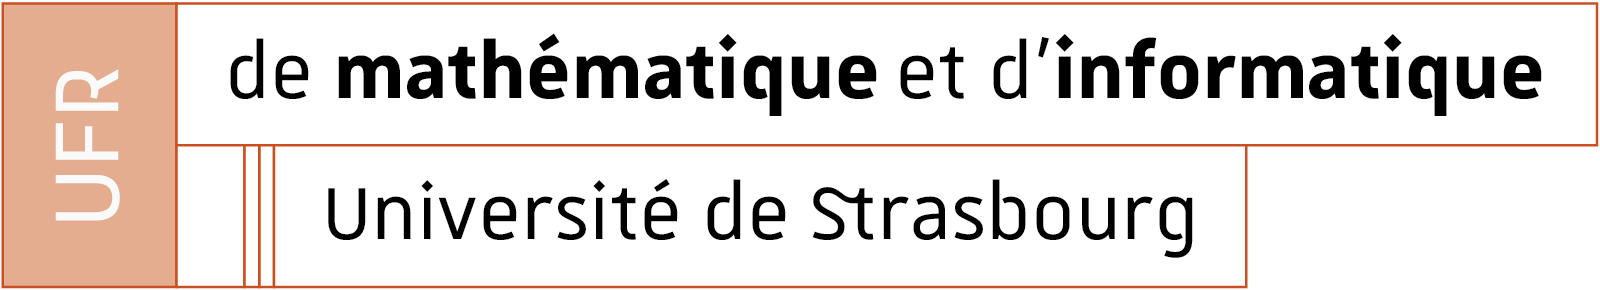
\includegraphics[width=0.8\textwidth]{images/logo_Uni.png}
  Project WP1 - Vegetation}
\author[SCP]{Giulio CARPI LAPI, Pierre-Antoine SENGER}

\begin{document}

\frame{\titlepage}

\begin{frame}{Introduction}

  \begin{figure}[h] % 'h' option tries to place the figure here
    \centering
    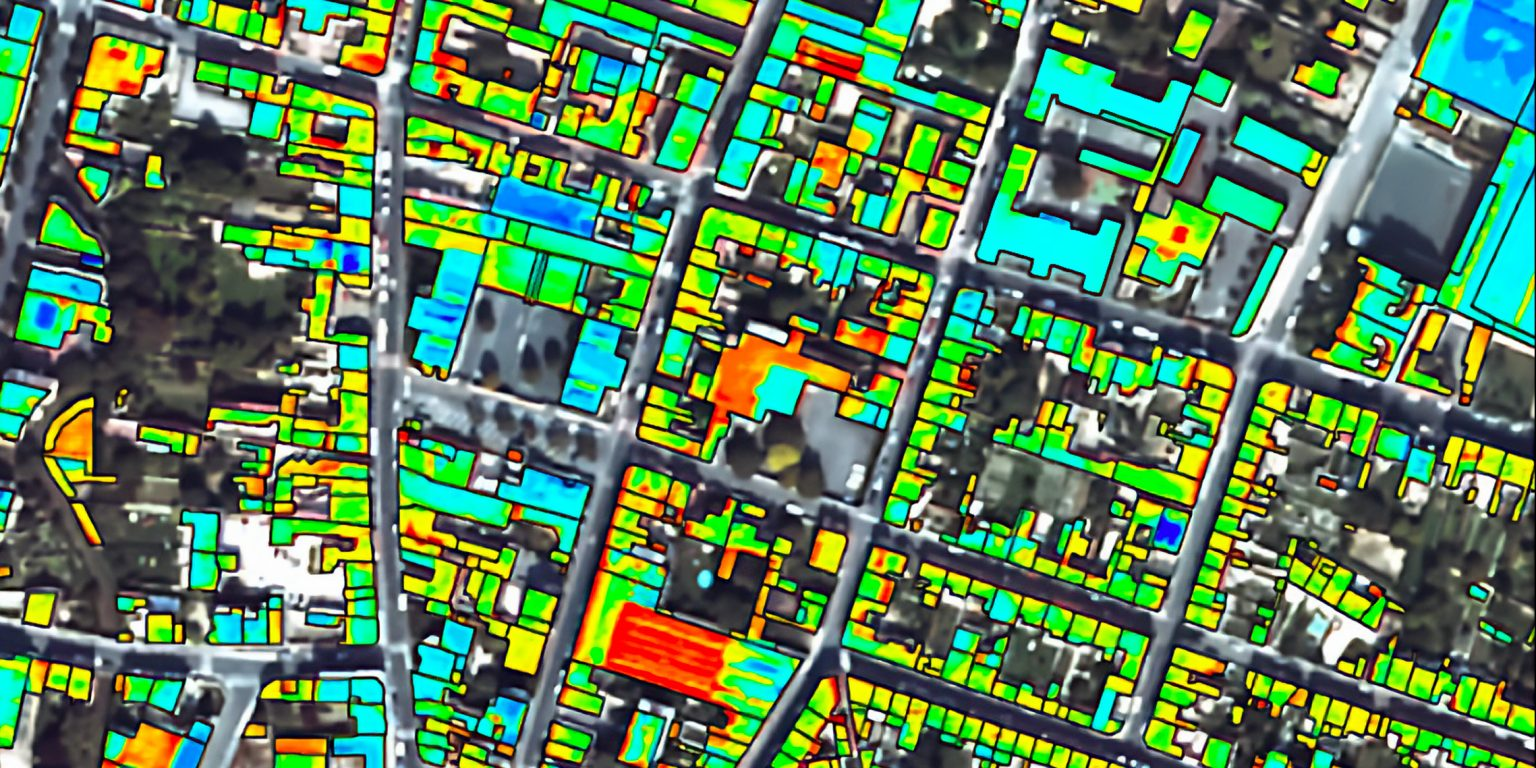
\includegraphics[width=1\textwidth]{images/thermographie-aerienne.jpg}
    \caption{aerial thermography of a city \cite{thermography}} % Caption for referencing
    \label{fig:thermographie} % Label for referencing
  \end{figure}

\end{frame}

\begin{frame}{trees in building thermal modeling}

    \begin{figure}[h] % 'h' option tries to place the figure here
      \centering
      \includegraphics[width=1\textwidth]{images/heat_street.png}
      \caption{thermal signature of a street \cite{street thermography}} % Caption for referencing
      \label{fig:3d_city_model} % Label for referencing
    \end{figure}

\end{frame}

\begin{frame}{Objectives}
  \begin{itemize}
    \item<1-> Access the OpenStreetMap database to extract information about trees location
    \item<2-> Create a 3D models library of trees
    \item<3-> Integrate the 3D models into the 3D city model
  \end{itemize}

\end{frame}
\begin{frame}{References}

\begin{thebibliography}{9}
  \bibitem{thermography} \url{https://www.somme.fr/services/appui-aux-collectivites/les-aides-du-departement/fonds-thermographie-aerienne/}
  \bibitem{street thermography} \url{https://theconversation.com/dou-vient-le-pouvoir-rafraichissant-des-arbres-en-ville-199906}
  \bibitem{osm-queries} \url{https://osm-queries.ldodds.com/tutorial}
  \bibitem{osm-learnoverpass} \url{https://osmlab.github.io/learnoverpass//en/}
\end{thebibliography}

\end{frame}

\end{document}
